\documentclass{article}\usepackage[]{graphicx}\usepackage[]{color}
%% maxwidth is the original width if it is less than linewidth
%% otherwise use linewidth (to make sure the graphics do not exceed the margin)
\makeatletter
\def\maxwidth{ %
  \ifdim\Gin@nat@width>\linewidth
    \linewidth
  \else
    \Gin@nat@width
  \fi
}
\makeatother

\definecolor{fgcolor}{rgb}{0.345, 0.345, 0.345}
\newcommand{\hlnum}[1]{\textcolor[rgb]{0.686,0.059,0.569}{#1}}%
\newcommand{\hlstr}[1]{\textcolor[rgb]{0.192,0.494,0.8}{#1}}%
\newcommand{\hlcom}[1]{\textcolor[rgb]{0.678,0.584,0.686}{\textit{#1}}}%
\newcommand{\hlopt}[1]{\textcolor[rgb]{0,0,0}{#1}}%
\newcommand{\hlstd}[1]{\textcolor[rgb]{0.345,0.345,0.345}{#1}}%
\newcommand{\hlkwa}[1]{\textcolor[rgb]{0.161,0.373,0.58}{\textbf{#1}}}%
\newcommand{\hlkwb}[1]{\textcolor[rgb]{0.69,0.353,0.396}{#1}}%
\newcommand{\hlkwc}[1]{\textcolor[rgb]{0.333,0.667,0.333}{#1}}%
\newcommand{\hlkwd}[1]{\textcolor[rgb]{0.737,0.353,0.396}{\textbf{#1}}}%

\usepackage{framed}
\makeatletter
\newenvironment{kframe}{%
 \def\at@end@of@kframe{}%
 \ifinner\ifhmode%
  \def\at@end@of@kframe{\end{minipage}}%
  \begin{minipage}{\columnwidth}%
 \fi\fi%
 \def\FrameCommand##1{\hskip\@totalleftmargin \hskip-\fboxsep
 \colorbox{shadecolor}{##1}\hskip-\fboxsep
     % There is no \\@totalrightmargin, so:
     \hskip-\linewidth \hskip-\@totalleftmargin \hskip\columnwidth}%
 \MakeFramed {\advance\hsize-\width
   \@totalleftmargin\z@ \linewidth\hsize
   \@setminipage}}%
 {\par\unskip\endMakeFramed%
 \at@end@of@kframe}
\makeatother

\definecolor{shadecolor}{rgb}{.97, .97, .97}
\definecolor{messagecolor}{rgb}{0, 0, 0}
\definecolor{warningcolor}{rgb}{1, 0, 1}
\definecolor{errorcolor}{rgb}{1, 0, 0}
\newenvironment{knitrout}{}{} % an empty environment to be redefined in TeX

\usepackage{alltt}
\usepackage[sc]{mathpazo}
\usepackage[T1]{fontenc}
\usepackage{geometry}
\geometry{verbose,tmargin=2.5cm,bmargin=2.5cm,lmargin=2.5cm,rmargin=2.5cm}
\setcounter{secnumdepth}{2}
\setcounter{tocdepth}{2}
\usepackage{url}
\usepackage[unicode=true,pdfusetitle,
 bookmarks=true,bookmarksnumbered=true,bookmarksopen=true,bookmarksopenlevel=2,
 breaklinks=false,pdfborder={0 0 1},backref=false,colorlinks=false]
 {hyperref}
\hypersetup{
 pdfstartview={XYZ null null 1}}


\newcommand{\R}{\texttt{R} }
\IfFileExists{upquote.sty}{\usepackage{upquote}}{}
\begin{document}
\title{Generating discrete morphological matrices with \R}

\author{Thomas Guillerme \\ t.guillerme@imperial.ac.uk}


\maketitle

This is just an informal note on what I've been working on on the Inapplicable data project and is now properly running.
Basically, prior to testing any algorithms dealing with inapplicable characters as we discussed last time, I spend some time developing some tools that you might find handy.
The following functions are stored in a \R ``package'' clumsily called \texttt{IterativeAlgo} (that ought to be changed in the near future).
They allow to generate some simulated yet realistic discrete morphological matrices and introduce some inapplicable characters.
These matrices just need a tree as an input and allow a certain number of parameters to be set by the user.

\section{Before starting}

The ``package'' is stored on my github page:

\begin{knitrout}
\definecolor{shadecolor}{rgb}{0.969, 0.969, 0.969}\color{fgcolor}\begin{kframe}
\begin{alltt}
\hlkwa{if}\hlstd{(}\hlopt{!}\hlkwd{require}\hlstd{(devtools))} \hlkwd{install.packages}\hlstd{(}\hlstr{"devtools"}\hlstd{)}
\hlkwd{install_github}\hlstd{(}\hlstr{"TGuillerme/Parsimony_Inapplicable/IterativeAlgo"}\hlstd{)}
\hlkwd{library}\hlstd{(IterativeAlgo)}
\end{alltt}
\end{kframe}
\end{knitrout}

A couple of packages are needed for running the functions and should install automatically.
If not, they can be installed from here
\begin{knitrout}
\definecolor{shadecolor}{rgb}{0.969, 0.969, 0.969}\color{fgcolor}\begin{kframe}
\begin{alltt}
\hlkwa{if}\hlstd{(}\hlopt{!}\hlkwd{require}\hlstd{(ape))} \hlkwd{install.packages}\hlstd{(}\hlstr{"ape"}\hlstd{)}
\hlkwa{if}\hlstd{(}\hlopt{!}\hlkwd{require}\hlstd{(ape))} \hlkwd{install.packages}\hlstd{(}\hlstr{"phangorn"}\hlstd{)}
\hlkwa{if}\hlstd{(}\hlopt{!}\hlkwd{require}\hlstd{(ape))} \hlkwd{install.packages}\hlstd{(}\hlstr{"phyclust"}\hlstd{)}
\hlkwa{if}\hlstd{(}\hlopt{!}\hlkwd{require}\hlstd{(ape))} \hlkwd{install.packages}\hlstd{(}\hlstr{"diversitree"}\hlstd{)}
\end{alltt}
\end{kframe}
\end{knitrout}

\section{Quick go through}

This is a quick example on how it works
\begin{knitrout}
\definecolor{shadecolor}{rgb}{0.969, 0.969, 0.969}\color{fgcolor}\begin{kframe}
\begin{alltt}
\hlkwd{library}\hlstd{(IterativeAlgo)}
\end{alltt}


{\ttfamily\noindent\color{warningcolor}{\#\# Warning in .doLoadActions(where, attach): trying to execute load actions without 'methods' package}}\begin{alltt}
\hlcom{## Setting the starting tree with 15 taxa as a random coalescent tree}
\hlstd{my_tree} \hlkwb{<-} \hlkwd{rcoal}\hlstd{(}\hlnum{15}\hlstd{)}

\hlcom{## Generating a matrix with 100 characters (85% binary and 15% three states) and}
\hlcom{## an equal rates model with a gamma rates distribution (0.5, 1) with no}
\hlcom{## invariant characters.}
\hlstd{my_matrix} \hlkwb{<-} \hlkwd{make.matrix}\hlstd{(}\hlkwc{tree} \hlstd{= my_tree,} \hlkwc{characters} \hlstd{=} \hlnum{100}\hlstd{,} \hlkwc{states} \hlstd{=} \hlkwd{c}\hlstd{(}\hlnum{0.85}\hlstd{,}
    \hlnum{0.15}\hlstd{),} \hlkwc{rates} \hlstd{=} \hlkwd{c}\hlstd{(rgamma,} \hlnum{0.5}\hlstd{,} \hlnum{1}\hlstd{),} \hlkwc{invariant} \hlstd{=} \hlnum{FALSE}\hlstd{)}

\hlcom{## Checking the matrix properties with a quick Maximum Parsimony tree search}
\hlkwd{check.matrix}\hlstd{(my_matrix, my_tree)}
\end{alltt}
\begin{verbatim}
## Most parsimonious tree search:
## Final p-score 155 after  1 nni operations
##                                     
## Maximum parsimony        155.0000000
## Consistency index          0.7032258
## Retention index            0.8601824
## Robinson-Foulds distance   6.0000000
\end{verbatim}
\begin{alltt}
\hlcom{## Adding 10 inapplicable characters (5 from characters and 5 from phylogeny)}
\hlstd{matrix_inap} \hlkwb{<-} \hlkwd{apply.inapplicables}\hlstd{(my_matrix,} \hlkwc{inapplicables} \hlstd{=} \hlkwd{c}\hlstd{(}\hlkwd{rep}\hlstd{(}\hlstr{"character"}\hlstd{,}
    \hlnum{5}\hlstd{),} \hlkwd{rep}\hlstd{(}\hlstr{"clade"}\hlstd{,} \hlnum{5}\hlstd{)), my_tree,} \hlkwc{invariant} \hlstd{=} \hlnum{FALSE}\hlstd{)}
\end{alltt}
\end{kframe}
\end{knitrout}

It is then possible to save this matrix in classic \texttt{nexus} format:

\begin{knitrout}
\definecolor{shadecolor}{rgb}{0.969, 0.969, 0.969}\color{fgcolor}\begin{kframe}
\begin{alltt}
\hlkwd{write.nexus.data}\hlstd{(matrix_inap,} \hlkwc{file} \hlstd{=} \hlstr{"test.nex"}\hlstd{)}
\end{alltt}
\end{kframe}
\end{knitrout}

\section{Details}
Details can be found for the three functions in their manuals:

\begin{knitrout}
\definecolor{shadecolor}{rgb}{0.969, 0.969, 0.969}\color{fgcolor}\begin{kframe}
\begin{alltt}
\hlopt{?}\hlstd{make.matrix}
\hlopt{?}\hlstd{check.matrix}
\hlopt{?}\hlstd{apply.inapplicables}
\end{alltt}
\end{kframe}
\end{knitrout}

Basically, \texttt{make.matrix} is really flexible and intakes a lot of different arguments to allow to simulate realistic matrix.
It has two implemented models: \texttt{"ER"} for Equal Rates (M\textit{k} model) or the \texttt{"HKY"} one which is the molecular HKY model but transforms pyrines in 0's and purimidines in 1's.
It can also intake some specific distribution for the rates or the substitutions, allowing to modify these basic models.

The \texttt{check.matrix} runs a quick MP tree using the \texttt{phangorn} parsimony algorithm.
It quickly calculates the parsimony score, the consistency and retention indices and, if a tree is provided (e.g. the tree used to generate the matrix) it calculates the Robinson-Foulds distance between the MP tree and the provided tree.

Finally, the interesting bit, the \texttt{apply.inapplicables} function transforms some of the characters states in the matrix into inapplicable tokens.
There are two way the algorithm replaces the states by a inapplicable token:
\begin{enumerate}
\item By selecting a ``pattern character'' in the matrix and linking it to a ``target character'' next to it.
The taxa with a randomly chosen state in the ``pattern character'' (e.g. 0) will then have an inapplicable character token for the ``target character''.
This is done by using the \texttt{"character"} argument and is meant to simulate data inapplicability that originates from the coder (i.e. I first coded the character ``tail'' - the ``pattern character'' - and then I coded ``tail color'' - the ``target character'').
\item By selecting a random clade or it's associated grade (i.e. everything that's not in the clade) and attributing inapplicable tokens for a given character to all the taxa present in that clade/grade.
This is done by using the \texttt{"clade"} argument and is meant to simulate data inapplicability that originates from the phylogeny (i.e. the deer's antlers that is present only in that clade).
\end{enumerate}

I was thinking it could be interesting to play with these two different character inapplicability ``origin'' and see if that influences anything.

\section{Good parameters for a good matrix}

I was testing the effect of different parameters on the ability to generate a ``realistic'' matrix (meaning not to different from the input tree with a consistency and retention index close to what's in the literature).
The matrix seems the most ``realistic'' with a starting coalescent tree, equal rates model with 0.85 binary characters and 0.15 three states characters (by the way, these proportion are extracted from observed data my Total Evidence paper \cite{GuillermeCooper}), a gamma distribution with a shape parameter ($\alpha$) of 0.5 and no scaling ($\beta$ = 1).

Something like that should give a decent matrix:
\begin{knitrout}
\definecolor{shadecolor}{rgb}{0.969, 0.969, 0.969}\color{fgcolor}\begin{kframe}
\begin{alltt}
\hlcom{## tree}
\hlstd{my_tree} \hlkwb{<-} \hlkwd{rcoal}\hlstd{(}\hlnum{15}\hlstd{)}
\hlcom{## matrix}
\hlstd{morpho_mat} \hlkwb{<-} \hlkwd{make.matrix}\hlstd{(my_tree,} \hlkwc{characters} \hlstd{=} \hlnum{100}\hlstd{,} \hlkwc{model} \hlstd{=} \hlstr{"ER"}\hlstd{,}
    \hlkwc{rates} \hlstd{=} \hlkwd{c}\hlstd{(rgamma,} \hlnum{0.5}\hlstd{,} \hlnum{1}\hlstd{),} \hlkwc{invariant} \hlstd{=} \hlnum{TRUE}\hlstd{)}
\hlcom{## }
\hlkwd{check.matrix}\hlstd{(morpho_mat, my_tree)}
\end{alltt}
\begin{verbatim}
## Most parsimonious tree search:
## Final p-score 75 after  0 nni operations
##                                    
## Maximum parsimony        75.0000000
## Consistency index         0.6666667
## Retention index           0.8717949
## Robinson-Foulds distance  4.0000000
\end{verbatim}
\end{kframe}
\end{knitrout}

\subsection{Testing the effect of the input tree}

\begin{figure}[!htbp]
\centering
   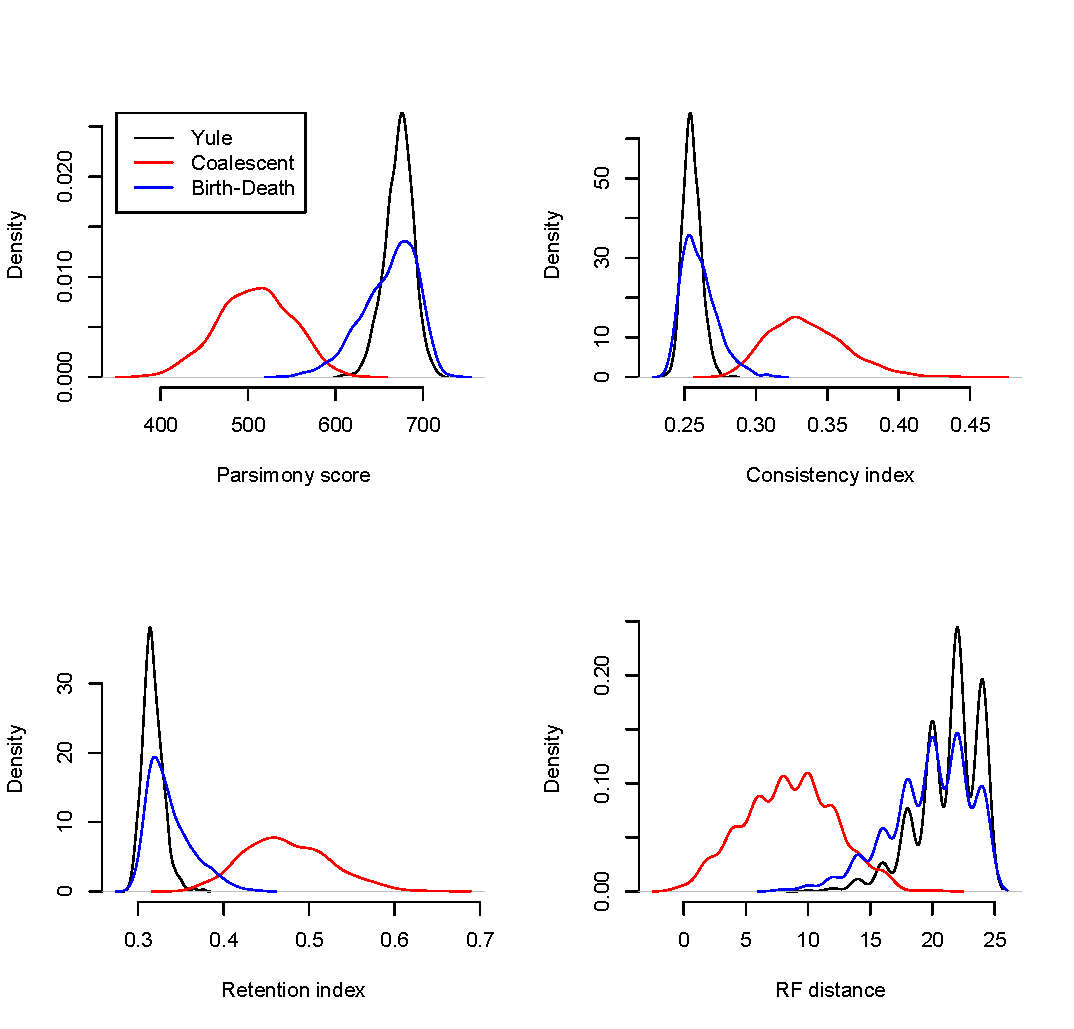
\includegraphics[width=1\textwidth]{Tree_effect.pdf}
\caption{Effect of a yule, coalescent or birth-death (with random $\lambda$ and $\mu$) starting tree.
The other parameters are fixed to be: \texttt{rates = c(rgamma, 0.5, 1)} and \texttt{model = "ER"}.
Simulations where repeated 1000 times per tree type.}
\label{Tree_effect}
\end{figure}

\subsection{Testing the effect of the model}

\begin{figure}[!htbp]
\centering
   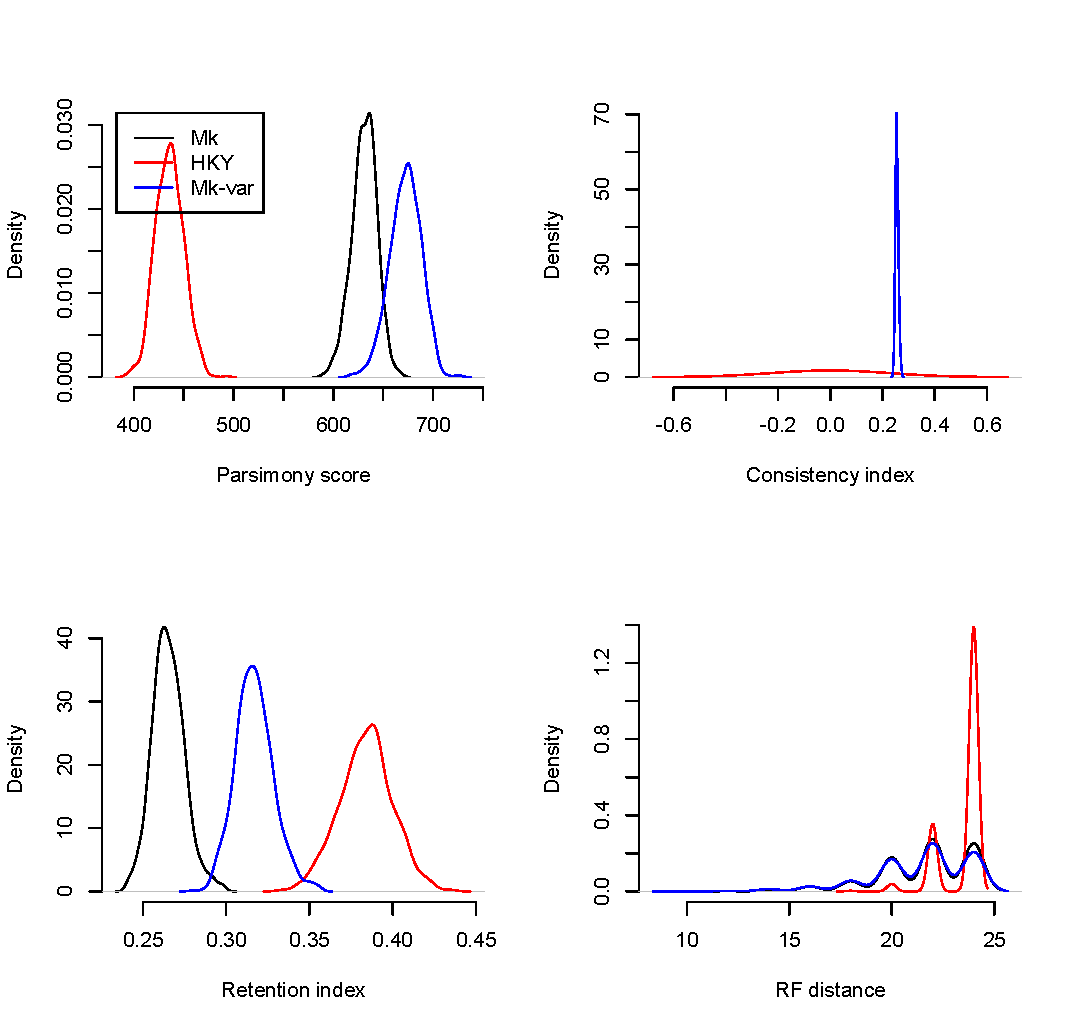
\includegraphics[width=1\textwidth]{Model_effect.pdf}
\caption{Effect of a Equal Rates (Mk), HKY (binary) or Mk with multiple states models.
The other parameters are fixed to be: \texttt{rates = c(rgamma, 0.5, 1)} and \texttt{tree = coalescent}.
Simulations where repeated 1000 times per model type.}
\label{Model_effect}
\end{figure}

\subsection{Testing the effect of the rates distribution}

\begin{figure}[!htbp]
\centering
   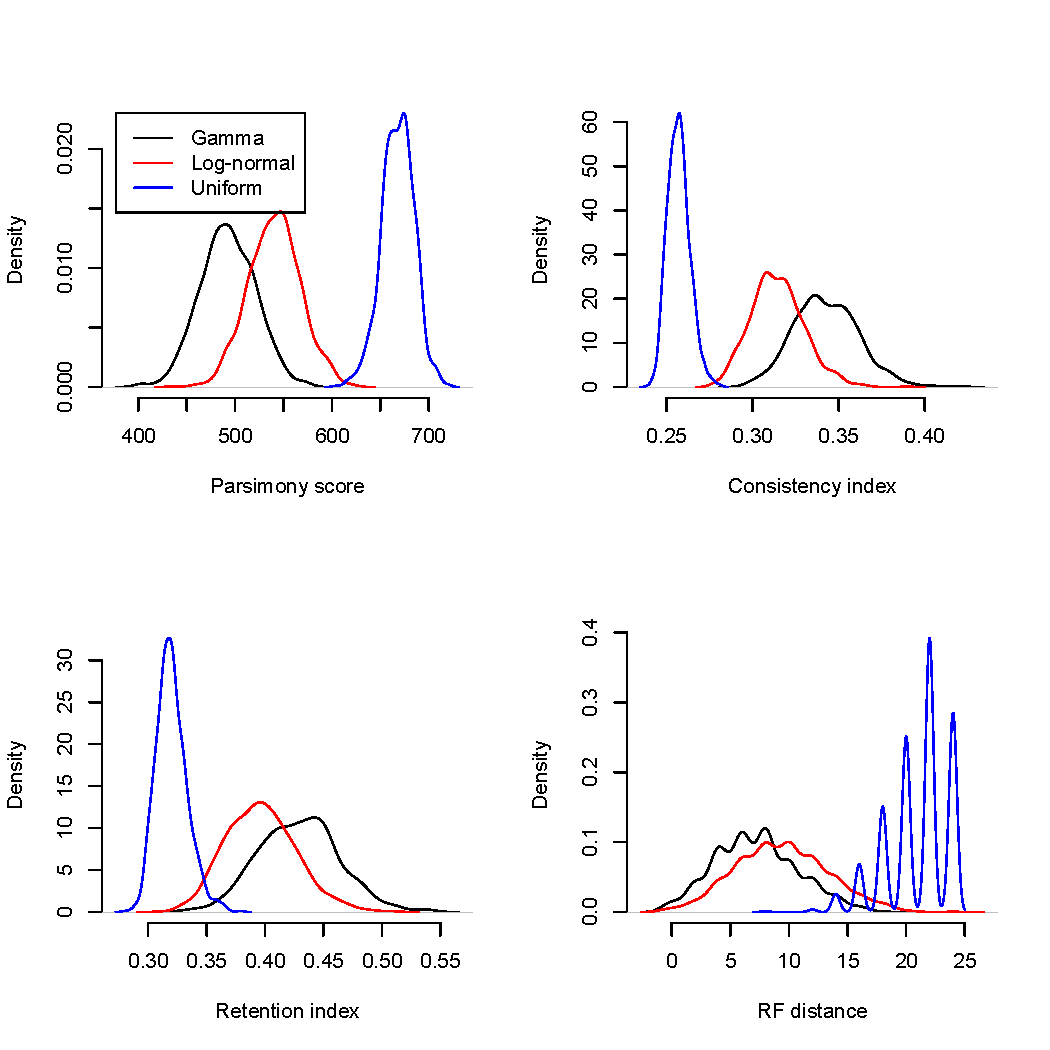
\includegraphics[width=1\textwidth]{Rate_distribution_effect.pdf}
\caption{Effect of a Gamma, Log-normal or Uniform rates distribution.
The other parameters are fixed to be: \texttt{model = "ER"} and \texttt{tree = coalescent}.
Simulations where repeated 1000 times per distribution type.}
\label{Rate_distribution_effect}
\end{figure}

\subsection{Testing the effect of the rates distribution shape}

\begin{figure}[!htbp]
\centering
   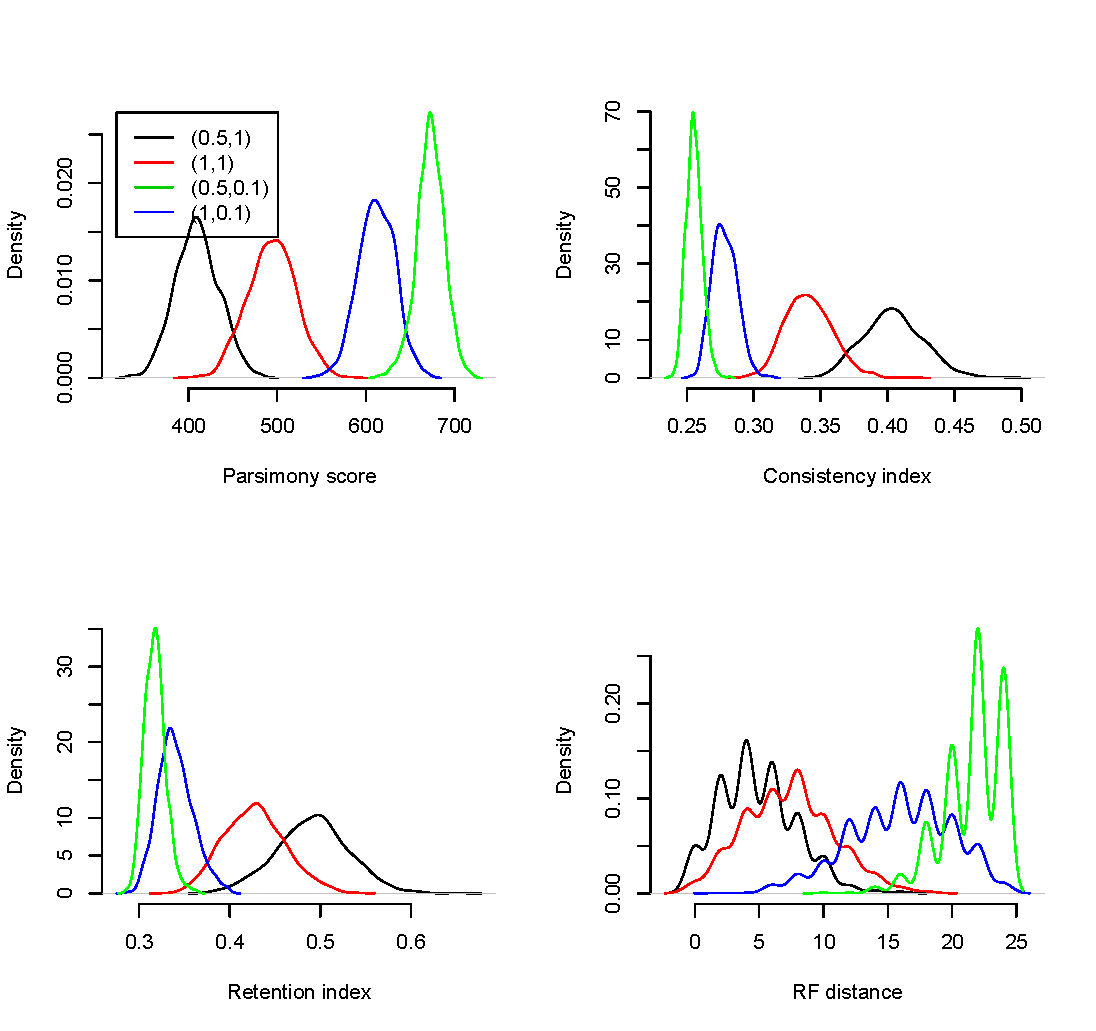
\includegraphics[width=1\textwidth]{Gamma_effect.pdf}
\caption{Effect of a Gamma distribution shape of $\alpha$=0.5 and $\beta$=1; $\alpha$=1 and $\beta$=1; $\alpha$=0.5 and $\beta$=0.1; and $\alpha$=1 and $\beta$=0.1.
The other parameters are fixed to be: \texttt{model = "ER"} and \texttt{tree = coalescent}.
Simulations where repeated 1000 times per shape type.}
\label{Gamma_effect}
\end{figure}

\bibliographystyle{vancouver}
\bibliography{References}


\end{document}
